\chapter{应用:血细胞形态学检测}
\oneline{在已上板验证的双板相机底座上,以"级联检测"架构把商用形态学分析仪
"检出—分类"链路中的检出半程移入千元级国产 FPGA:前端负责框选、裁剪、上传
(确定性毫秒级,上行链路已由千兆 UDP 实现),上位机负责细分类与图库陈列。
\textbf{本章为应用设计章:检测类新增功能尚未实施,全部指标为设计目标并注明依据。}}

\section{背景与临床价值}

血细胞形态学检查(白细胞五分类计数,原始细胞、浆细胞、有核红细胞等异常细胞的检出)
是血液病筛查的核心手段,当前两端都有痛点:人工镜检慢(每片数十分钟)、依赖经验、
主观差异大;自动化形态学分析仪(CellaVision 及国产同类)检出与分类全自动,但设备
数十万元级,难以在基层普及。任务可以拆成"找细胞"与"认细胞"两半——前者只需要几何与
颜色特征(染色后白细胞核深染、体积大、密度低,经典图像处理即可高召回定位),后者必须
神经网络(核形、颗粒、核浆比等语义特征)。这两半恰好对应"廉价实时硬件"与"通用算力"
的最优分工。

本系统的检测对象是 \textbf{Giemsa(瑞氏—吉姆萨)染色血涂片}:血液推片经甲醇固定后,
以含天青与伊红的 Romanowsky 类染液染色——细胞核、核染质等嗜碱性结构被染成蓝紫色,
血红蛋白与胞浆等嗜酸性结构被染成粉红色。染色后,白细胞核深染、体积明显大于红细胞与
血小板,与背景形成稳定的"颜色—尺寸"对比;中性粒/淋巴/单核/嗜酸/嗜碱五类白细胞亦依
核形与颗粒着色得以区分。这一对比正是"找细胞"可以交给经典图像处理的物理基础:
FPGA 以核深染条件二值化提出候选,实时框选染色细胞,再按框裁剪 96$\times$96 细胞
截图,经千兆网送上位机细分类。

\section{级联检测架构}

前端(FPGA)负责框选、裁剪、上传——哑而快、确定性毫秒级;上位机(PC)负责细分类
与图库展示——算力充足、可迭代升级。这与商用系统的成熟形态一致,本方案的创新点在于
\textbf{把"找"的一半放进百元级国产 FPGA 流水线,使单套系统成本下降 1$\sim$2 个
数量级};同时系统上电即跑、检出不依赖 PC,识别结果驱动 IO 报警,构成"采集—处理—
决策—执行"的完整闭环。系统级数据流如图~\ref{fig:apparch} 所示。

\begin{figure}[H]\centering
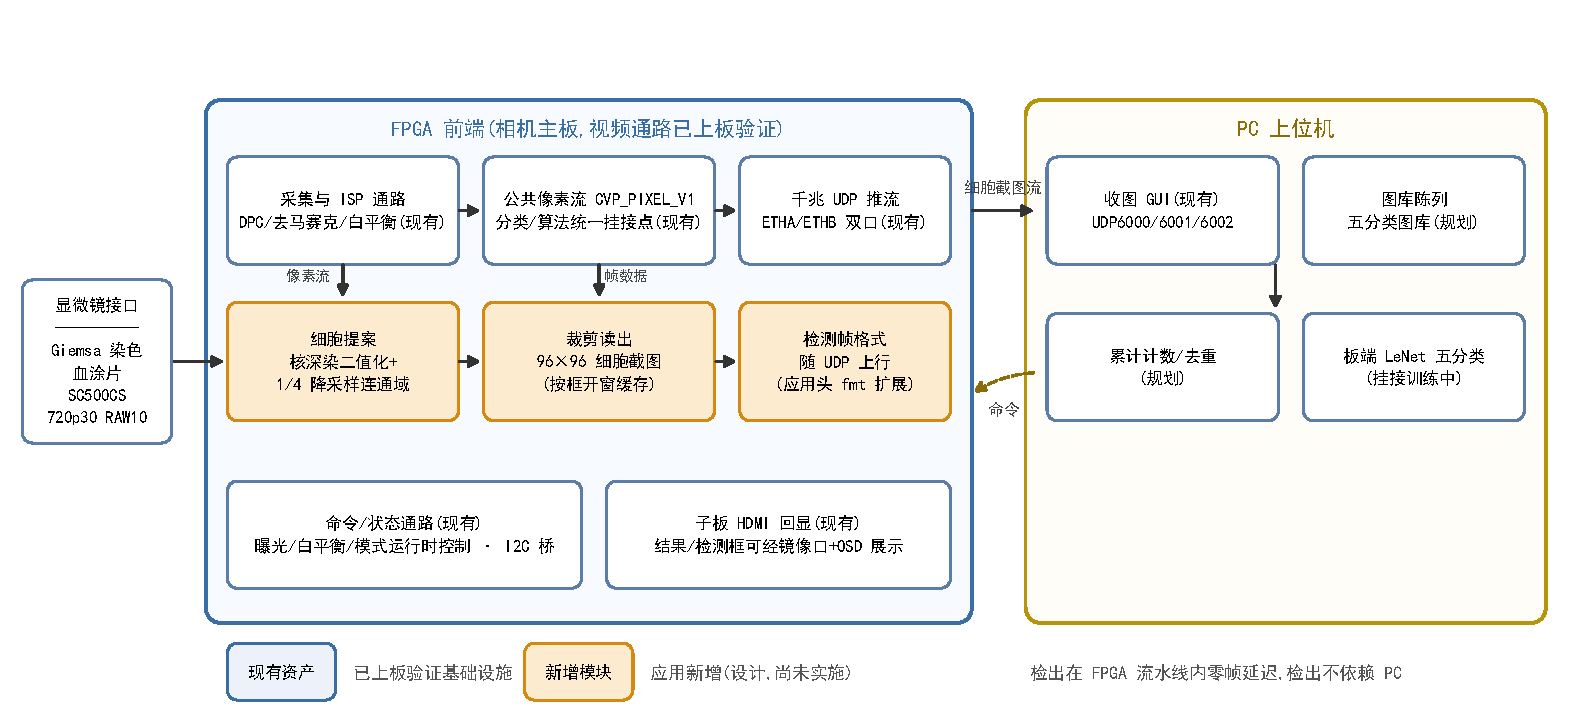
\includegraphics[width=\textwidth]{figs/fig_app_arch.pdf}
\caption{血细胞形态学检测系统级联架构(蓝框 = 已上板验证资产,橙框 = 应用新增模块)}
\label{fig:apparch}
\end{figure}

\section{FPGA 侧新增工作量}

在定版底座上,工程量集中在两个新增 RTL 模块(细胞提案、裁剪读出),上行链路已由
千兆 UDP 推流实现,其余全部复用现有设施:

\begin{table}[h!]\centering\small
\caption{FPGA 侧新增工作量}
\begin{tabular}{p{2.6cm}p{9.2cm}p{2.6cm}}
\toprule
模块 & 做法 & 资源估计 \\
\midrule
细胞提案 & 核深染条件二值化(现有二值化模式改造) $\to$ 1/4 降采样域单趟连通域标记
(标签表存 ERAM) $\to$ 面积/圆度门限筛选 & $<$5\% LUT + 数块 ERAM \\
裁剪读出 & 第 $k$ 帧锁存框坐标 $\to$ 在直通链路上按框开窗缓存 96$\times$96 像素
(行/列计数命中窗口) $\to$ 检测帧格式随 UDP 上行 & 复用为主 \\
去重触发 & 质心注册表自动去重;演示阶段可按键触发整批上传(零逻辑) & $<$1\% LUT \\
\bottomrule
\end{tabular}
\end{table}

\section{复用资产映射}

定版的每一块基础设施在这个应用里都有明确落点,这是"级联架构工作量可控"的依据:

\begin{table}[h!]\centering\small
\caption{复用资产映射(定版底座)}
\begin{tabular}{p{5.4cm}p{9cm}}
\toprule
现有资产 & 在应用中的角色 \\
\midrule
全视频通路(DPC/去马赛克/色彩校正,位级与上板验证) & 提案与裁剪的数据来源,不需要改动 \\
公共像素流接口(CVP\_PIXEL\_V1) & \textbf{分类网络的统一挂接点}:128\,bit 像素字
含坐标/帧身份/模式号元数据,即插即用不动主链路 \\
千兆 UDP 推流(UDP 6000,1920 包/帧)+ ETHA/ETHB 双口 & 裁剪细胞截图与检测结果
的上行链路,\textbf{已实现};检测结果亦可经镜像口驱动子板 OSD 展示 \\
命令/状态通路(UDP 6001/6002) & 曝光/白平衡运行时控制已实现;检测帧格式可在此
扩展 \\
PC 预览 + 子板 HDMI 回显 & 两路并行观察视野(PC/显示器);主板本地 DSI 支路已于 v30 裁剪 \\
二值化等像素级模式 & 细胞提案(核深染掩膜)的实现基础 \\
按键模式切换 & 扫描触发、批管理的人机接口 \\
仿真回归体系(主板 RTL/Python + 子板记分板) & 新增模块沿用同一验证方法论 \\
\bottomrule
\end{tabular}
\end{table}

\section{上位机与分类器}

上位机经网口收包、重组裁剪图,送分类器后在图库 UI 陈列(参考商用形态:左侧实时
视野、右侧分类图库、底部累计计数),并做跨视野去重;收图 GUI 与命令/状态链路
(UDP 6000/6001/6002)已随主板工程交付。分类器目标为板端部署的 LeNet 架构轻量级神经
网络:网络轻量、算力与存储开销低;能否与当前主板工程的剩余资源及时序预算相匹配
仍需在接入真实模型后重新综合、布线和评估,完成五种白细胞的图像
分类;分类挂接点即公共像素流接口(CVP\_PIXEL\_V1),训练以 PBC 公开数据集
(Acevedo 等,约 1.7 万张已裁剪单细胞图、8 类)为起点,再用自采染色图微调。
该方案另有一个数据集红利:FPGA 的裁剪输出天然构成"位置已标定"的细胞图库,
随使用持续积累训练数据。

\needspace{10\baselineskip}
\section{关键指标(设计目标)}

\textbf{下表全部为设计目标与文献依据,不是实测结果}:提案召回阈值将在阶段 0 用 BCCD
数据集仿真标定,分类精度按文献口径,带宽按千兆链路核算。

\begin{table}[H]\centering\small
\caption{关键指标(设计目标)}
\begin{tabular}{p{3.2cm}p{6.4cm}p{4.6cm}}
\toprule
维度 & 指标(目标) & 依据 \\
\midrule
检出实时性 & 30\,fps 流水线内完成,零帧延迟 & 提案在 100\,MHz 写侧流水线内,
1 像素/拍 \\
上传带宽 & 裁剪 96$\times$96 RGB = 27.6\,KB;千兆 UDP 每秒上千张 & 推流链路
实测 1920 包/帧稳定 \\
单张端到端延迟 & $\leq$0.4\,s(检出 0 + 裁剪 $\leq$1 帧 + 传输 + 分类 $<$50\,ms) &
静态视野场景 \\
扫描规模 & 每视野 5$\sim$15 个白细胞;累计 200 个约 1$\sim$2 分钟 & 与商用系统演示
节奏一致 \\
提案召回 & 目标 $\geq$95\%(阈值换召回,误报由上位机分类器剔除) & BCCD 数据集仿真
验证 \\
分类精度 & 主类(五分类)$\geq$95\% & PBC 数据集文献 \\
FPGA 资源 & 与 LeNet 轻量网络共占空闲资源,仍待实现后核算 & v38 主板布线
占用 Slice 10944/21216 (51.58\%),ERAM 51/108、DSP 16/40;可用余量不得直接等同于
可用于网络的预算,接入模型后必须重新评估资源与时序 \\
\bottomrule
\end{tabular}
\end{table}

\needspace{10\baselineskip}
\section{风险与对策}

\begin{table}[H]\centering\small
\caption{风险与对策}
\begin{tabular}{p{3.4cm}p{2.6cm}p{8.2cm}}
\toprule
风险 & 影响 & 对策 \\
\midrule
提案漏检(漏检 = 漏诊) & 系统性 & 阈值放宽换召回 + 面积窗滤血小板簇;BCCD 仿真定
阈值,召回作硬指标验收 \\
色彩保真(分型依赖染色色度) & 分类精度 & 白平衡已支持四模式 + 网络运行时控制
(第 4 章),视野内放白色参考块锚定;进阶:裁剪改传 RAW10(免插值色偏),上位机
统一处理 \\
异常类别训练数据稀缺(原始细胞/浆细胞/有核 RBC) & 扩展受限 & 演示版做五分类 +
"异常可疑"兜底类(低置信度标黄人工复核),异常检出作为扩展方向 \\
30\,fps 推流高带宽占用 & 上传并发 & 检测帧与视频帧分端口/分格式;必要时降帧 \\
\bottomrule
\end{tabular}
\end{table}

\needspace{10\baselineskip}
\section{实施计划}

\begin{table}[H]\centering\small
\caption{实施计划}
\begin{tabular}{cp{7.4cm}p{3.6cm}p{2.4cm}}
\toprule
阶段 & 内容 & 产出/判据 & 状态 \\
\midrule
0 & 软件闭环:BCCD 提案召回实验 + 上位机原型 & 召回率—误报率曲线定阈值;UI 定版 &
AE 控制律/GUI 已完成,余项进行中 \\
1 & FPGA 提案 + 框选 + 计数 & 实时框选白细胞,仿真逐位对拍通过 & 待启动(需板) \\
2 & 裁剪读出 + 千兆上行 + 上位机接通 & 图库逐个生成分类细胞 & 上行链路已就绪 \\
3 & LeNet 五分类 + 累计计数、去重、异常标黄 & 200 细胞累计扫描全流程演示 &
网络训练进行中 \\
4(可选) & 多前端汇聚演示 & 网络化形态 & 规划 \\
\bottomrule
\end{tabular}
\end{table}

\noindent 阶段 0 不需要任何硬件投入,即可验证全部关键假设(召回可达性、阈值、
上位机形态);阶段 1 起依赖上板(部署流程见各工程 README)。

\section{结论}

\textbf{技术可行}:所需算法(二值化/连通域/裁剪/统计)均为 FPGA 流水线的经典问题,
上行链路已在定版中实现,无技术空白点;\textbf{价值成立}:把商用形态学分析仪
"检出—分类"链路中的检出半程移入千元级国产 FPGA,单套成本降 1$\sim$2 个数量级,
且检出部分确定性毫秒级延迟、可 7$\times$24 运行;\textbf{风险可控}:主要风险
(提案召回、色彩保真)均有量化验收手段与既定对策,全部关键假设可在零硬件投入的
阶段 0 先行验证;\textbf{叙事完整}:从"实时视觉前端平台"到"血细胞形态学检测"的
垂直应用,展示同一硬件底座(实时流式处理 + 网络命令控制 + 千兆上行 + 双板三路
显示)的可复用性。
